\chapter{Binding C++ and SpiderMonkey}\todo{properName}
\label{chap:LanguageBindingCPPJS}

This chapter shows how \myProperName{C++} elements like declarations and types can be exposed to \myProperName{Mozilla SpiderMonkey} to be used from scripts. \myProperName{SpiderMonkey} is the name of \myProperName{Mozilla}'s implementation of the \myProperName{ECMAScript} programming language standard, which is most commonly known as \myProperName{JavaScript}. The terms \myProperName{JavaScript} and \myProperName{ECMAScript} will be used interchangebly, whereas \myProperName{SpiderMonkey} refers to the concrete \myProperName{Mozilla} implementation.\\
Binding \myProperName{C++} elements to other programming languages like \myProperName{Python}\footnote{\myProperName{Python}: \url{http://www.python.org/}}, \myProperName{Lua}\footnote{\myProperName{Lua}: \url{http://www.lua.org/}} or other \myProperName{JavaScript} implementations, e.g. \myProperName{V8}\footnote{\myProperName{V8}: \url{http://code.google.com/p/v8/}}, will be similar in many aspects and specific differences will depend upon the existing elements of the target language.

The information in this chapter presumes knowledge about the \myProperName{C++} programming language, its elements, type system and class-based inheritance.

Language binding between \myProperName{SpiderMonkey} and \myProperName{C++} could fill a book on its own. Thus, only the most important aspects will be presented in this chapter.

\section{\myProperName{JavaScript}/\myProperName{ECMAScript}}
\label{sec:JavaScript}

\myProperName{JavaScript} is a weakly typed object-oriented programming language with garbage collection. 

As it is a feature-rich language, only the most important aspects will be presented in this section. More information can be found in \myProperName{Mozilla}'s \myProperName{JavaScript} guide\footnote{\myProperName{JavaScript} guide: \url{https://developer.mozilla.org/en/JavaScript/Guide}} or in various books like \myAuthorName{David Flanagan}'s \myBookName{JavaScript: The Definite Guide} or \myAuthorName{Douglas Crockford}'s \myBookName{JavaScript: The Good Parts}.

\myProperName{JavaScript} values belong to one of six basic types: boolean, number, string, \mySCName{undefined}, \mySCName{null} and object.\\
Number, string and boolean are primitive types. So are \mySCName{null} and \mySCName{undefined}, which both represent the absence of value. All these types are immutable.\todo{ref}\\
Objects are basically mutable collections of name-value-pairs, known as properties or \mySlang{members}. They can be seen as hash-maps or associative arrays. Object properties can be accessed using bracket-syntax (e.g. \mySCName{var foo["bar"] = 3;}) or dot-notation (e.g. \mySCName{var foo.bar = 3;}). An \mySCName{Array} is a specialized type of \myProperName{JavaScript} object.\\
Functions are special objects that have source code associated and thus can be invoked. Being objects, functions can have properties and can even be passed as parameters.

\SingleSpacing
\begin{lstlisting}[language=JavaScript, caption=Types in \myProperName{JavaScript}]
// primitive types
var aNumber = 34.9;
var aBoolean = true;
var aString = "Some text!";
var aNullValue = null;
var anUndefinedValue; // standard type for variables that have 
                      // not been initialized
var anotherUndefinedValue = undefined;

// object types
var anObject = {};
anObject.foo = "bar";
anObject.subObject = { foo: "bar"};

var anArray = [];

function aFunction(param)
{
	return param * 3;
}

aFunction.someProperty = "Functions are objects, too!";
\end{lstlisting}
\OnehalfSpacing

When being passed as parameters or assigned to variables, primitive values are passed by value / copy-assigned, whereas objects (including functions) are passed/assigned by reference.\\
\myProperName{JavaScript} thus has no notion of pointers and changes made to primitive values passed as function parameters will not have any effect on the original value.

There are two kinds of properties: value properties and accessor properties. A value property simply contains any type of value (e.g. a number or function). Accessor properties have a getter and setter function associated that can perform additional computation when getting or setting a value. They are used just like ordinary data properties.

\SingleSpacing
\begin{lstlisting}[language=JavaScript, caption=Properties in \myProperName{JavaScript}, label=JSTypes]
var obj = {
	// value properties
	aValue: 3,
	aValue_Function: function(){ this.aValue *= 2; },
	
	// an accessor property
	get accessorProp(){ return this.aValue + 3; },
	set accessorProp(val){ this.aValue = val - 3; }
};

obj.aValue = 4;        // --> obj.aValue is 4
obj.aValue_Function(); // --> obj.aValue is 8
obj.accessorProp = 6;  // --> obj.aValue is 3 (6-3)
\end{lstlisting}
\OnehalfSpacing

Functions like \mySCName{aValue\_Function} in \myRefListing{JSTypes} do not strictly belong to the object they are declared in. Their execution context or scope (which can be referred to using the \mySCName{this} keyword from within the function) is determined at run-time and usually refers the object through which the function is called. With the help of a function object's \mySCName{call} method, an execution context can be forced.

\SingleSpacing
\begin{lstlisting}[language=JavaScript, caption=Execution context of functions]
// obj1 declares the function
var obj1 = {
	name: "Paul",
	sayHello: function (){ return "Hello, I am " + this.name; }
}

// obj2 borrows the function (and additionally renames it)
var obj2 = {};
obj2.name = "John";
obj2.sayHello_renamed = obj1.sayHello; 

var obj3 = { name: "Ringo" };

obj1.sayHello();          // --> "Hello, I am Paul"
obj2.sayHello_Renamed();  // --> "Hello, I am John"

// forcing the execution context
obj1.sayHello.call(obj3); // --> "Hello, I am Ringo"

\end{lstlisting}
\OnehalfSpacing

\subsection{Inheritance}
\label{sec:JSInheritance}

The prototypical inheritance mechanism used in \myProperName{JavaScript} differs vastly from the class-based inheritance already known from \myProperName{C++} and \myProperName{Java}. In a class-based inheritance the class defines a design contract that created instances adhere to.\\
\myProperName{JavaScript} uses prototypes instead. A prototype object is an ordinary \myProperName{JavaScript} object, from which other objects inherit properties. When \myProperName{JavaScript} looks up a property of an object, the object is checked if it does have an own property with the name. If not, its prototype is checked for the property. If this does not have it either, the prototype's prototype is checked and so on up its hierarchy. This hierarchy is called the prototype chain.\\
The prototype of an object is saved as an internal property ([[Prototype]]) that can not be set after object creation and can only be accessed using \linebreak\mySCName{Object.getPrototypeOf(anObject)}. Some implementations add the non-standard \linebreak\mySCName{\_\_proto\_\_} property for accessing the prototype.\\
If a property with the same name exists on an object that has a prototype, then it shadows the prototype's property.

\SingleSpacing
\begin{lstlisting}[language=JavaScript, caption=Prototypes]
var aPrototype = { aProp: "Prop of prototype" };
aPrototype.aProp; // --> "Prop of prototype"

// creating an object with aPrototype as the prototype
var anInstance = Object.create(aPrototype);
Object.getPrototypeOf(anInstance) == aPrototype // --> true

anInstance.aProp; // --> "Prop of prototype"

// shadowing
anInstance.aProp = "Prop of instance";
anInstance.aProp; // --> "Prop of instance"
\end{lstlisting}
\OnehalfSpacing

\subsubsection{Classes}
\label{sec:JSClasses}

Classes can be mimicked in \myProperName{JavaScript} with the help of constructor functions. Whenever a function is called with the \mySCName{new} operator, a new object (instance) is created. This object's internal [[Prototype]] property is set to the \mySCName{prototype} property of the function. These two are not to be confused. The \mySCName{this} keyword will refer to the created instance and can be used to define properties on the instance, for example \mySCName{name} in \myRefListing{JSClasses}. The \mySCName{sayHello} function will be shared by all instances, as it is defined on the prototype, whereas \mySCName{name} only exists on the instances themselves.

\SingleSpacing
\begin{lstlisting}[language=JavaScript, caption=Classes in \myProperName{JavaScript}, label=JSClasses]
function Person(name)
{
	this.name = name;
}

Person.prototype.sayHello = function()
{
	return "Hi, my name is (what?), my name is " + this.name;
}

var anInstance = new Person("Slim Shady");
anInstance.sayHello();
// --> "Hi, my name is (what?), my name is Slim Shady"
\end{lstlisting}
\OnehalfSpacing

For creating inheritance chains, the internal [[Prototype]] property of a function's \linebreak\mySCName{prototype} object must reference another function's \mySCName{prototype} object. If a base constructor function initializes members, then it must be called explicitly from the subclass constructor function with the help of the function object's \mySCName{call} method.

\SingleSpacing
\begin{lstlisting}[language=JavaScript, caption=Prototype-based inheritance in \myProperName{JavaScript}, label=JSClasses]
function Base()
{
	this.baseMember = 3;
}

Base.prototype.doSomething = function(){ return this.baseMember * 3;}

function SubClass()
{
	// call Base constructor with call (and without new)
	Base.call(this);
	this.subclassMember = "Another member";
}

// assigning a new prototype object with [[Prototype]] Base.prototype
SubClass.prototype = Object.create(Base.prototype);
// resetting the constructor property
SubClass.prototype.constructor = SubClass;

var instance = new SubClass();
instance.doSomething(); // --> 9 (3 * 3)

\end{lstlisting}
\OnehalfSpacing

\vspace{10pt}
\begin{figure}[h] % h = here
	\centering
		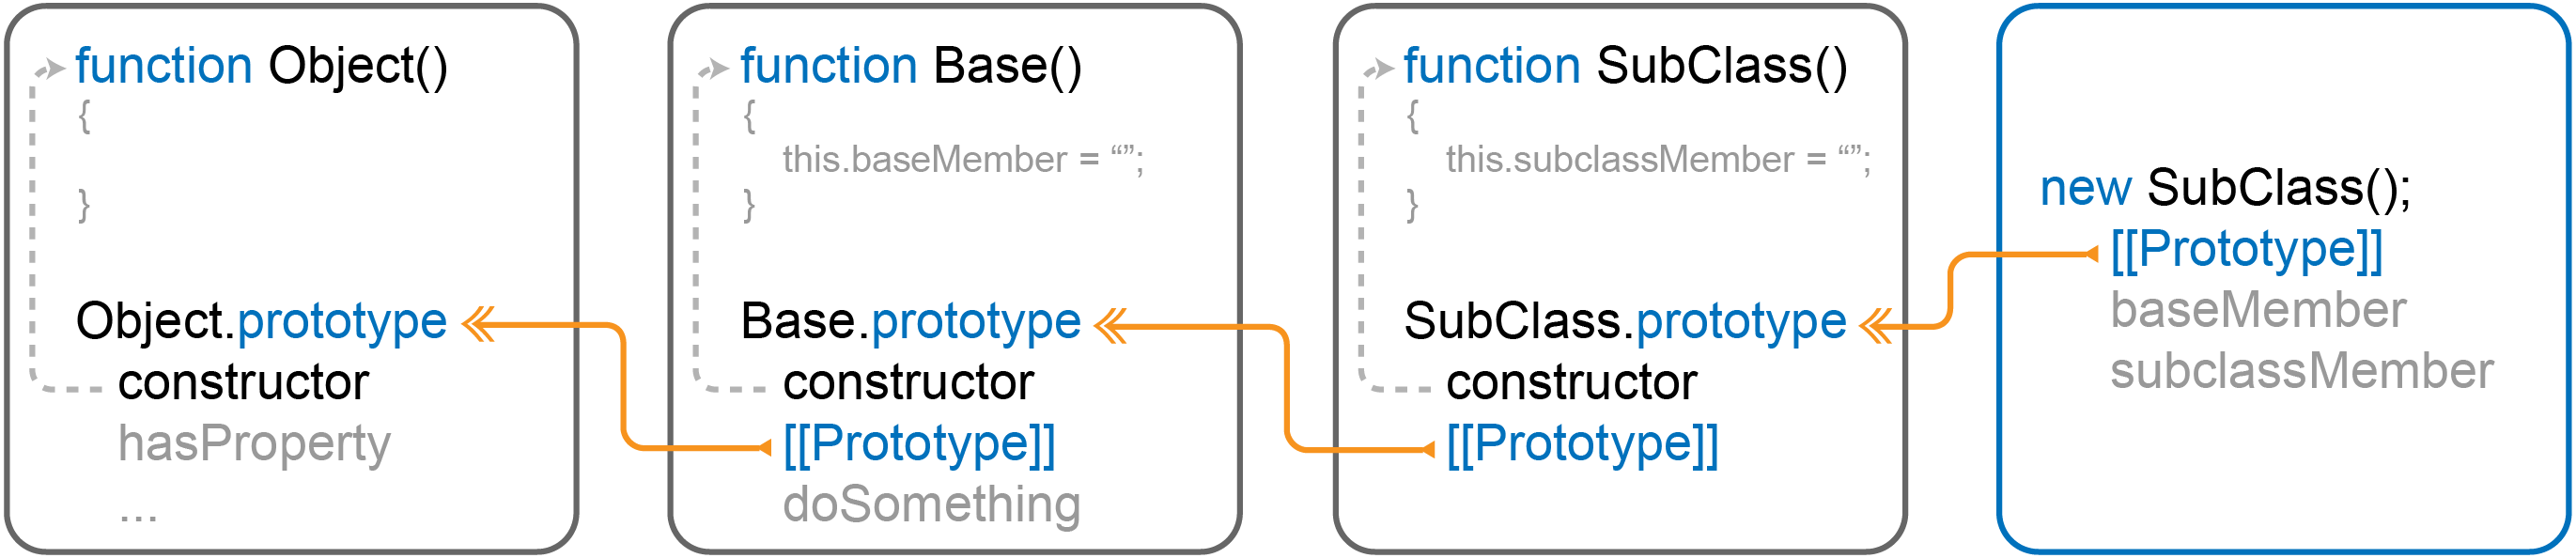
\includegraphics[scale=0.32]{Images/PrototypeChain.png}
	\caption{The prototype chain}
	\label{fig:InheritanceWrapping}
\end{figure}

\subsubsection{Mixins}
\label{sec:Mixins}

Multiple inheritance is not supported in \myProperName{JavaScript}, but can be mimicked to a certain degree by borrowing functions. This concept is also called \textbf{mixin}.

\SingleSpacing
\begin{lstlisting}[language=JavaScript, caption=Mixins in \myProperName{JavaScript}, label=JSMixins]
function BaseA(){}
BaseA.prototype.funcA = function(){}

function BaseB(){}
BaseB.prototype.funcB = function(){}

function SubClass()
{
	BaseA.call(this);
	BaseB.call(this);
}

// borrowing functions / mixing in
SubClass.prototype.funcA = BaseA.prototype.funcA;
SubClass.prototype.funcB = BaseB.prototype.funcB;

// creating an instance
var instance = new SubClass();
instance.funcA();
instance.funcB();
\end{lstlisting}
\OnehalfSpacing

\section{\myProperName{SpiderMonkey}}

\myProperName{SpiderMonkey} comes in the form of a shared library exposing a \myProperName{C} API, which can be used to interact with the \myProperName{JavaScript} virtual machine. This API is also known as \myProperName{JSAPI}. Due to the length of this thesis, the API can only be presented in excerpts. A full overview is given at the \myProperName{Mozilla Developer Network JSAPI} reference\footnote{\myProperName{JSAPI} reference: \url{https://developer.mozilla.org/en/SpiderMonkey/JSAPI_Reference}}.

A \mySCName{JSRuntime} is an instance of the virtual machine. A \mySCName{JSContext} is a single environment within a \mySCName{JSRuntime}, in which all objects and values live. One \mySCName{JSRuntime} can have multiple \mySCName{JSContext}s. Each context has a global object. Objects are exposed as \mySCName{JSObject}.

A \myProperName{JavaScript} value is expressed as a \mySCName{jsval}. \mySCName{jsval} contains information about the type of the value (number, boolean, etc.). For strings and objects, the \mySCName{jsval} stores the pointer to the \mySCName{JSString} or \mySCName{JSObject}. For all other types, the data is saved in the \mySCName{jsval} itself. \mySCName{jsval}s occur at several places in \myProperName{JSAPI}, for example when defining properties, for parameter values or return values.\\
\myProperName{SpiderMonkey} provides utility macros/functions for checking the type of a \mySCName{jsval} \linebreak(e.g. \mySCName{JSVAL\_IS\_OBJECT}) and its content (e.g. \mySCName{JSVAL\_TO\_OBJECT}) or for creating \mySCName{jsval}s from the corresponding \myProperName{SpiderMonkey} \myProperName{C++} types (e.g. \mySCName{OBJECT\_TO\_JSVAL}).\\
When converting between \mySCName{jsval}s and \myProperName{C++} types, type checking needs to be performed. The \myProperName{C++} compiler that compiles the glue code will perform this task, when converting \textbf{to} \mySCName{jsval}, as the conversion functions only accept the correct type. When converting a \mySCName{jsval} to a \myProperName{C++} type, the current type of the \mySCName{jsval} needs to be checked manually first. If the \myProperName{JSAPI} user, for example, tries to retrieve a \mySCName{JSObject} from a \mySCName{jsval} that contains a boolean value, the behaviour of the code is undefined and will probably lead to a run-time failure like a crash. Thus type checking and error handling play an important role and are explained in further detail in \myRefSection{sec:ErrorHandling}.\\
\myProperName{SpiderMonkey} also provides utility functions for automatic conversion of types according to the \myProperName{ECMAScript} standard. If, for example, a boolean is passed to a function that expects a string, the conversion would create a string from the boolean - either \mySCString{true} or \mySCString{false}. These conversion functions are less performant, but allow for a greater range of input values without reporting errors. It has to be said though, that automatic conversion can lead to unexpected program behaviour in places where the user would expect an error.\\
Most of the conversion functions take a \mySCName{JSContext} as the parameter.

A \mySCName{JSObject} has a \mySCName{void} pointer that \myProperName{JSAPI} users can use for storing any kind of private data. This will be useful for storing pointers of \myProperName{C++} classes.

\section{Boolean Values}

Boolean values can be converted between \mySCName{jsval}s and the \myProperName{C++} boolean type using \mySCName{JSVAL\_TO\_BOOLEAN} and \mySCName{BOOLEAN\_TO\_JSVAL}. \mySCName{JS\_ValueToBoolean} can be used for automatic conversion. If the function returns false, the given \mySCName{jsval} could not be converted.

\SingleSpacing
\begin{lstlisting}[language=C++, caption=Conversion of boolean values]
bool cppValue = true;

// A) to jsval
jsval jsValue = BOOLEAN_TO_JSVAL(cppValue);

// B) from jsval - strict
if(JSVAL_IS_BOOLEAN(jsValue))
	cppValue = JSVAL_TO_BOOLEAN(jsValue)
else
	// error handling
	
// C) from jsval - using automatic conversion
if(!JS_ValueToBoolean(context, jsValue, &cppValue))
	// error handling
\end{lstlisting}
\OnehalfSpacing

\section{Number Values}

\myProperName{ECMAScript} supports only a single number type. There is no distinction between integers and floating point values.\\
\myProperName{SpiderMonkey} internally makes a difference and provides macros like \mySCName{JSVAL\_TO\_INTEGER}, which will lead to an undefined result if the \mySCName{jsval} contains a double value. Thus, \myProperName{SpiderMonkey} also provides generalized versions for converting between \myProperName{C++} types and the \myProperName{JavaScript} numbers, which should be used instead:

\begin{itemize}\addtolength{\itemsep}{-0.5\baselineskip}
	\item \mySCName{JS\_NewNumberValue}: creates a number \mySCName{jsval} from integer or floating point value
	\item \mySCName{JSVAL\_IS\_NUMBER}
	\item \mySCName{JS\_ValueToNumber}: converts to \mySCName{double}
	\item \mySCName{JS\_ValueToECMAInt32}
	\item \mySCName{JS\_ValueToECMAUint32}
	\item \mySCName{JS\_ValueToUint16}
\end{itemize}

When converting to integers, the number value is rounded according to the \myProperName{ECMAScript} standard.

Usage of these macros and functions is similar to converting boolean values.

\section{Strings}

\mySCName{STRING\_TO\_JSVAL}, \mySCName{JSVAL\_IS\_STRING}, \mySCName{JSVAL\_TO\_STRING} and \mySCName{JS\_ValueToString} (with automatic conversion) can be used for converting between \mySCName{jsval} and \mySCName{JSString}.

\myProperName{JavaScript} strings are sequences of 16 bit wide characters. In \myProperName{SpiderMonkey} such a character is defined as a \mySCName{jschar} and \mySCName{JSString} is a sequence of \mySCName{jschar}s. A \mySCName{jschar} is UTF-16.

\mySCName{JSString}s can be converted to null-terminated \myProperName{C++} character arrays using \linebreak\mySCName{JS\_EncodeString}. The caller is responsible for managing the created memory. \linebreak\mySCName{JS\_NewStringCopyZ} can be used to convert a null-terminated character array to a \mySCName{JSString}.

\SingleSpacing
\begin{lstlisting}[language=C++, caption=Conversion of strings]
const char* cppStr = "This is a null-terminated string";

// A) to jsval
JSString* jsStrToScript = JS_NewStringCopyZ(context, cppStr);
if(!jsStrToScript)
	// error handling
jsval jsValue = STRING_TO_JSVAL(jsStrToScript);

// B) from jsval - using automatic conversion
JSString* jsStrFromScript = JS_ValueToString(context, jsValue);
if(!jsStrFromScript)
	// error handling
	
char* cppStrFromScript = JS_EncodeString(context, jsStrFromScript);
if(!cppStrFromScript)
	// error handling
	
// ... using the char* ...
// ...

// cleaning up
if(cppStrFromScript)
	delete[] cppStrFromScript;
\end{lstlisting}
\OnehalfSpacing

To handle \mySCName{std::string}, its \mySCName{c\_str} method needs to be used to retrieve a \mySCName{const char*}. \mySCName{std::string} can be constructed from character arrays.

\subsection{Unicode}

As \mySCName{jschar} is UTF-16, \mySCName{JSString}s can be created from and converted to 16-bit unicode strings.\\
\mySCName{JS\_NewUCStringCopyZ} creates a \mySCName{JSString} from an array of \mySCName{jschar}s, whereas \linebreak\mySCName{JS\_GetStringCharsZ} returns an array of \mySCName{jschar}s from a \mySCName{JSString}.

The \myProperName{JSAPI} user has to do the conversion from his unicode character type to \mySCName{jschar} and vice versa.\\
\myProperName{C++}'s wide character type \mySCName{wchar\_t} is not well suited for this task, as its size is compiler-specific. It is allowed to be at least 8 bit. On \myProperName{VC++} it is 16 bit, on GCC even 32 bit.\\
\myProperName{C++11} introduces new character types for unicode characters: \mySCName{char16\_t} and \mySCName{char32\_t}. Having a fixed width, \mySCName{char16\_t} should be the same as a \mySCName{jschar} on all platforms and thus be best suited for conversion between unicode strings and \mySCName{JSString}.

\section{Namespaces}

In \myProperName{C++} namespaces exist for grouping other elements. In \myProperName{JavaScript} the same task can be achieved by creating a hierarchy of \mySCName{JSObject} instances. \mySCName{JS\_DefineObject} can be used to define an object property on another object.

\SingleSpacing
\begin{lstlisting}[language=C++, caption=Wrapping a namespace]
namespace Outside {
	namespace Inside {
		// ... declare functions, classes, etc.
	}
}

// somewhere in the glue code ...
// defining jsOutside on the global object
JSObject* jsOutside = JS_DefineObject(context, 
                             globalObject, "Outside", NULL, NULL, 0);
if(!jsOutside)
	// error handling
else {
	// defining jsInside on jsOutside
	JSObject* jsInside = JS_DefineObject(context, 
                             jsOutside, "Inside", NULL, NULL, 0);
	if(!jsInside)
		// error handling
	else {
		// ... wrap content of "Inside": functions, classes, etc.
	}
}
\end{lstlisting}
\OnehalfSpacing

\section{Functions}
\label{sec:Functions}

Functions are generally wrapped with the help of wrapper functions of the function type \mySCName{JSNative}. The wrapper function has to convert the parameters from \myProperName{JavaScript} values to \myProperName{C++} values, call the wrapped function and convert its return value to a \myProperName{JavaScript} value. If errors occur (for example when parameters of wrong types have been passed) or exceptions are thrown somewhere in the called \myProperName{C++} code, these have to be handled and the function will return \mySCName{false} to indicate a pending \myProperName{JavaScript} exception.

\SingleSpacing
\begin{lstlisting}[language=C++, caption=A simple wrapper function]
float getFloat(bool param1, int param2);

JSBool getFloat_wrapper(JSContext *cx, uintN argc, jsval *vp)
{
	if(argc < 2)
		// throw JS exception: not enough parameters (return false)

	// handling parameters
	jsval* args = JS_ARGV(cx, vp);

	bool param1;
	if(!JS_ValueToBoolean(cx, args[0], &param1))
		// throw JS exception: wrong parameter type (return false)
	
	int param2;
	if(!JS_ValueToNumber(cx, args[1], &param2))
		// throw JS exception: wrong parameter type (return false)

	// calling function
	try {	
		int cppResult = getFloat(param1, param2);
		
		// setting return value
		if(!JS_NewNumberValue(cx, cppResult, &JS_RVAL(cx, vp)))
			// throw JS exception: could not create return value
		
	} catch (...) {
		// forward C++ exception as JS exception and return false
	}

	// no errors occurred
	return true;
}
\end{lstlisting}
\OnehalfSpacing

\mySCName{JSNative} gets three arguments. The \mySCName{JSContext} of the current call, the number of passed arguments (\mySCName{argc}) and an array of \mySCName{jsval}s named \mySCName{vp}. \mySCName{vp} contains the execution context (the \mySCName{this}), the passed arguments and a \mySCName{jsval} for the return value. The execution context can be retrieved using \mySCName{JS\_THIS(cx, vp)}. \mySCName{JS\_ARGV(cx, vp)} returns a pointer to the first parameter \mySCName{jsval}. \mySCName{JS\_RVAL(cx, vp)} retrieves the \mySCName{jsval} that will be the return value of the function call.

Primitive types are converted as explained in the previous chapters. The conversion of class types is explained in \myRefSection{sec:StructsAndClasses}. \\
Primitive types, including strings, are immutable. As such functions that take a reference or pointer to an immutable type (e.g. \mySCName{int\&} or \mySCName{char[]}) and try to change the value of the parameter during the call (sometimes referred to as \mySlang{out-parameter}) will not effect the actual \myProperName{JavaScript} parameter. The wrapper functions of such procedures must be written differently and the call from script-side will need to pass a mutable type (e.g. a \mySCName{JSObject}) whose members refer to the immutable parameters.

The wrapper function needs to be defined on a \mySCName{JSObject} (e.g. the global object) so it can be used from script. There are multiple ways to do this, for example with \mySCName{JS\_DefineFunction}:

\SingleSpacing
\begin{lstlisting}[language=C++, caption=Defining a function]
JSFunction* func = JS_DefineFunction(context, 
        someJSObject,      // the JSObject* to define on
        "getFloat",        // name of the function
        getFloat_Wrapper,  // wrapper function
        2,                 // number of expected arguments 
        JSPROP_ENUMERATE); // flags
        
if(!func)
	// error handling
\end{lstlisting}
\OnehalfSpacing


\subsection{Overloaded Functions}
\label{sec:OverloadedFunctions}

\myProperName{JavaScript} does not support overloaded functions per se. Instead, a function can inspect the parameters it was called with and behave according to the number and types of parameters passed.

When wrapping overloaded functions, the wrapper function can decide on the \myProperName{C++} function to call by checking the \mySCName{argc} argument for the number of parameters. For overloaded functions with the same number of parameters, it can check the type of parameter with the functions \myProperName{JSAPI} provides (e.g. \mySCName{JSVAL\_IS\_NUMBER}, etc.).

Problems can arise for functions that overload on a type that has the same representation in \myProperName{JavaScript}, for example \mySCName{float} and \mySCName{double}. Given a number value, there is no way to decide on the correct overload implementation in such a case.

\subsection{Default Arguments}

Similar to overloaded functions, the number of actually passed parameters needs to be checked to decide on how many can be converted and passed to the \myProperName{C++} function.

It is open to debate what should happen if a wrong parameter type is passed for a parameter that has a default value. As a valid function call is technically possible, the wrong type could simply be ignored and the default value used. This silent fail may lead to unintended behaviour though and thus is highly questionable.

\section{Classes}
\label{sec:StructsAndClasses}

The wrapping of custom types and inheritance hierarchies comes with many possible pitfalls.\\
\myProperName{C++} classes can be best mapped to \myProperName{JavaScript} constructor functions, as explained in \myRefSection{sec:JSClasses}. \myProperName{SpiderMonkey} provides the structure \mySCName{JSClass} and the function \mySCName{JS\_InitClass} for performing this task.

A \mySCName{JSClass} object contains the name of a class, some flags and a set of \mySlang{hooks} - functions that are called by the \myProperName{JavaScript} engine on specific events. One of these \mySlang{hooks} is the finalize operation. This will be called, when a \mySCName{JSObject}, that was created from this class, is garbage collected.\\
The most important flag to set on the \mySCName{JSClass} is \mySCName{JSCLASS\_HAS\_PRIVATE}. Setting this flag allows the objects created from the class to have a private data field. This field of type \mySCName{void*} will be used to store the instances of a wrapped \myProperName{C++} class.\\
The function \mySCName{JS\_InitClass} creates a prototype \mySCName{JSObject} from a given \mySCName{JSClass} and defines functions and properties on it. It defines the \myProperName{JavaScript} constructor function for the wrapped class on the given scope object. It takes a constructor \mySCName{JSNative}, which will be called, when instances are created in script via \mySCName{new}. This constructor usually creates an instance of the wrapped \myProperName{C++} class and saves it as the private data.

\SingleSpacing
\begin{lstlisting}[language=C++, caption=Initializing a class, label=lst:InitClass]
void finalize(JSContext *cx, JSObject *obj)
{
	// called upon garbage collection
}

JSClass jsClass = {
	"SampleClassWrap",    // Name of the class
	JSCLASS_HAS_PRIVATE,  // Flags
	JS_PropertyStub,      // Default hooks
	JS_PropertyStub, 
	JS_PropertyStub, 
	JS_StrictPropertyStub,
	JS_EnumerateStub, 
	JS_ResolveStub, 
	JS_ConvertStub, 
	finalize              // finalize operation
};

JSObject* jsPrototype;

// called when instance created via new
JSBool constructor(JSContext *cx, uintN argc, jsval *vp)
{
	// create the JavaScript object with the class and prototype
	JSObject* obj = JS_NewObject(cx, &jsClass, jsPrototype, NULL);
	if (!obj)
		// error handling
	else
	{
		// create instance of C++ class and save it as private data
		if(!JS_SetPrivate(cx, obj, new ::SampleClass()))
			// error handling
		else
			// set the object as the return value
			JS_SET_RVAL(cx, vp, OBJECT_TO_JSVAL(obj));
	}
	
	return true;
}

// initializing the class on a given scope JSObject
jsPrototype = JS_InitClass(context, 
		scope,       // scope JSObject to define constructor function on	
		NULL,        // parent prototype
		&jsClass,    // the used JSClass
		constructor, // constructor function
		0,           // expected parameters of constructor
		NULL,        // instance properties
		NULL,        // instance functions
		NULL,        // static properties
		NULL         // static functions
	);
\end{lstlisting}
\OnehalfSpacing

\myRefListing{lst:InitClass} shows the initialization of the constructor function \mySCName{SampleClassWrap} along with its prototype. \mySCName{SampleClassWrap} wraps the \myProperName{C++} class \mySCName{SampleClass}. New instances can be created from script via \mySCName{new SampleClassWrap()}, which will lead to new instances of \mySCName{SampleClass} being created. The given code does not expose any members, as the call to \mySCName{JS\_InitClass} passes \mySCName{NULL} for all properties and functions.

\subsection{Private Data}
\label{sec:PrivateData}

When wrapping member functions and fields, the corresponding wrapper code needs to retrieve the instance of the \myProperName{C++} class from the \mySCName{this} \mySCName{JSObject}'s private data. Within a \mySCName{JSNative}, the \mySCName{this} \mySCName{JSObject} can be retrieved by using \mySCName{JS\_THIS\_OBJECT}.

As functions can be borrowed and the execution context be forced in \myProperName{JavaScript}, there is no guarantee that the \mySCName{JSObject}'s private data contains an instance of the expected class. Thus type checking has to be performed to validate the correct type of the private data and convert it from the \mySCName{void*}. Calling instance functions on unchecked values can lead to crashes or undefined behaviour.

When saving an instance as a private data \mySCName{void} pointer, type information is \mySlang{lost} and is impossible to be retrieved - not even using RTTI and \mySCName{dynamic\_cast}. \myProperName{C++} itself gives us no means of checking the data to be of a specific type. Thus, for performing type checking, the \mySCName{JSObject} itself is checked, whether it is of a specific \mySCName{JSClass}. An object of class \mySCName{SampleClassWrap} is guaranteed to hold an instance of \mySCName{SampleClass} as its private data - and nothing else. \myProperName{SpiderMonkey} provides two important functions for performing such type checks.\\
\mySCName{JS\_GetInstancePrivate} returns the private data of a \mySCName{JSObject}, but checks the object to be of a given \mySCName{JSClass}. If the check fails, it returns \mySCName{NULL}.\\
\mySCName{JS\_HasInstance} checks a \mySCName{JSObject} (to be precise: a \mySCName{jsval}), whether it is an instance of a given constructor function by checking the whole prototype chain. Therefore it is better suited when wrapping inheritance chains.\\
If these checks succeed, a private data value can safely be converted to the correct \myProperName{C++} type using \mySCName{static\_cast}.

Another possible way of type checking is to save the type information along with the private data. This concept will be presented in \myRefSection{sec:GenericWrapper}.

\myProperName{SpiderMonkey} provides another way of storing private data. A \mySCName{JSClass} can be initialized to give its \mySCName{JSObject}s a fixed number (between 0 and 255) of reserved slots for \mySCName{jsval}s. Though being subject to GC, these slots are not exposed to script and can be used for any purpose.

\subsection{Constructors}

Because a constructor is just a \mySCName{JSNative}, \myProperName{JavaScript} parameters are passed to it like to any other wrapped function. As explained in \myRefSection{sec:OverloadedFunctions}, the correct constructor implementation for creating the \myProperName{C++} instance can be chosen based on the number and types of arguments.

As can be seen in \myRefListing{lst:InitClass}, the constructor's task is to create a \mySCName{JSObject} instance that will be returned. The created \myProperName{C++} instance will be stored as the private data of the \mySCName{JSObject}.

\subsection{Wrapping Existing Instances}

Already existing instances of \myProperName{C++} classes that the user wants to access from script can be wrapped similarly to the creation within a constructor. A new \mySCName{JSObject} with the proper \mySCName{JSClass} and prototype needs to be created and the existing instance stored as the private data.

\SingleSpacing
\begin{lstlisting}[language=C++, caption=Wrapping an instance]
SampleClass* getInstance();
SampleClass getInstanceCopy();

JSObject* wrapObj = JS_NewObject(context, 
			&sampleClass_JSClass,           // JSClass
			 sampleClass_Prototype, NULL);  // Prototype JSObject
			 
if (!wrapObj)
	// error handling
else
{
	// store the instance
	if(!JS_SetPrivate(context, wrapObj, getInstance()))
		// error handling
}

\end{lstlisting}
\OnehalfSpacing

\subsubsection{Wrapping Copies}
\label{sec:WrappingCopies}

Stack-allocated return values (e.g. the return of \mySCName{getInstanceCopy}) need to be wrapped differently, as they will be destroyed at the end of the current code block. A new instance has to be heap-allocated using the copy constructor. This instance will then be wrapped instead of the original return value.

\subsection{Member Functions}

The wrapping of member functions works similar to the wrapping of free functions as explained in \myRefSection{sec:Functions}.

For the function call to work, the class instance needs to be retrieved from the private data of the \mySCName{this} \mySCName{JSObject} as explained in \myRefSection{sec:PrivateData}. Type checking has to be performed.

\subsection{Fields}
\label{sec:Fields}

In \myProperName{C++}, data members (fields) are often not declared as \mySCName{public}, but will instead be accessed using getter and setter functions.

In both cases, either a \myProperName{JavaScript} value property or accessor property can be created. Depending on what kind of property is chosen, the behaviour may be different.

Exposing getters and setters as properties (e.g. \mySCName{obj.setVal(x)} becomes \mySCName{obj.val = x}) will give the wrapped class a more natural feeling, when being used from the scripting language, as function call syntax is removed.

\subsubsection{Accessor Properties}

For accessor properties, wrapper functions for getting and setting the property need to be provided. The setter function can be omitted, making the property read-only. The wrapper functions are of type \mySCName{JSPropertyOp} and work similarly to a \mySCName{JSNative}.\\
The \myProperName{C++} instance needs to be retrieved from the given \mySCName{JSObject}'s private data. A getter would retrieve the field or call the \myProperName{C++} getter function and then set it as the return \mySCName{jsval}. A setter would set the field or call the \myProperName{C++} setter function.

\SingleSpacing
\begin{lstlisting}[language=C++, caption=Glue code for accessor properties]
class SampleClass
{
	public:
		bool m_member;
		
		bool getMember();
		void setMember(bool val);
};

// glue code
JSBool member_getter_wrap(JSContext* cx, JSObject* obj, jsid id, 
                          jsval* vp)
{
	// retrieving SampleClass* from obj's private data
	// SampleClass* instance = ... (omitted from example)
	
	*vp = BOOLEAN_TO_JSVAL(instance->m_member);
	// or via getter function: 		
	// *vp = BOOLEAN_TO_JSVAL(instance->getMember());

	return true;
}

JSBool member_setter_wrap(JSContext* cx, JSObject* obj, jsid id, 
                          JSBool strict, jsval* vp)
{
	// retrieving SampleClass* from obj's private data
	// SampleClass* instance = ... (omitted from example)
	if(JSVAL_IS_BOOLEAN(*vp))
	{
		instance->m_member = JSVAL_TO_BOOLEAN(*vp);
		// or via setter function: 		
		// instance->setMember(JSVAL_TO_BOOLEAN(*vp));
	}
	else
		// error handling

	return true;
}
\end{lstlisting}
\OnehalfSpacing

Accessor properties can be defined by passing them to \mySCName{JS\_InitClass} or using \linebreak\mySCName{JS\_DefineProperty} on a \mySCName{JSObject}.

\subsubsection{Value Properties}
\label{sec:ValueProperties}

Non-primitive non-settable fields can be stored as value properties. Struct or class instances that are completely stored inside a class and only have a getter function fall into this category. This also applies to pointers that are guaranteed to not be replaced.

\SingleSpacing
\begin{lstlisting}[language=C++, caption=Fields usable for value properties]
class ClassA
{
	public:
		ClassB& getUsable();   // usable for value properties
	private:
		ClassB  m_usable;  
		ClassB* m_maybeUsable; // only if pointer is not changed
		int m_primitive;       // not usable

};
\end{lstlisting}
\OnehalfSpacing

When creating a value property, the field's actual value (e.g. the \mySCName{ClassB} instance) is wrapped into a \mySCName{JSObject}. This is then defined as a property on the \mySCName{JSObject} that wraps the \mySCName{ClassA} instance. After property definition, the \mySCName{ClassA} instance is not used anymore for accessing the field. That is why the field needs to be non-replaceable. If the field's value could be replaced, the \myProperName{JavaScript} property would still refer to the old instance.

In contrast to functions and accessor properties, value properties for non-static members are defined on the instance-wrapping \mySCName{JSObject} and not on the prototype. Thus \mySCName{JS\_DefineProperty} needs to be called, wherever the corresponding \mySCName{JSObject} is created - for example in the constructor or a function that wraps an existing instance.

\SingleSpacing
\begin{lstlisting}[language=C++, caption=Defining a value property]
ClassA* classA = new ClassA();
JSObject* classAWrap = // (omitted): create JSObject, set private data

JSObject* classBWrap = wrapClassBInstance(classA->getUsable());

// defining the property
if(!JS_DefineProperty(context, 
           classAWrap,                  // JSObject to define on
           "usable",                   // property name
           OBJECT_TO_JSVAL(classBWrap), // value to define
           NULL, NULL,
           JSPROP_ENUMERATE)            // flags
	// error handling
\end{lstlisting}
\OnehalfSpacing

Value properties can also be defined lazily with the help of the \mySCName{JSClass}'s resolve hook. The resolve hook is called, when a property is not found on an object.

Because type checking is only performed when defining the property and the holding instance (of \mySCName{ClassA}) is not needed afterwards, access to value properties has better performance than using accessor properties.

\subsection{Static Members}

Static data members and functions are wrapped similar to fields and functions. As they are static, they make no use of the \mySCName{this} object. When calling \mySCName{JS\_InitClass}, static properties and functions can be passed. \myProperName{JavaScript} has no real concept of static members as there is no distinction between classes and instances. When declaring ``static'' properties using \mySCName{JS\_InitClass}, these are simply defined on the created constructor function, so access to static members looks similar to \myProperName{C++}. Contrary to \myProperName{C++}, it is not possible to access a static member from within an instance using \mySCName{this} - static members always have to be accessed using the constructor function object.

\subsection{Inheritance}

The inheritance mechanism described in \myRefSection{sec:JSInheritance} can also be used in glue code. \mySCName{JS\_InitClass} accepts a \mySCName{JSObject} that will be set as the internal [[Prototype]] property of the constructor function's prototype.

The \myProperName{C++} class hierarchy does not necessarily need to be replicated on the \myProperName{JavaScript} side. \myRefFigure{fig:InheritanceWrapping} shows that base class members can also just be defined on the subclass wrapper.

\begin{figure}[h] % h = here
	\centering
		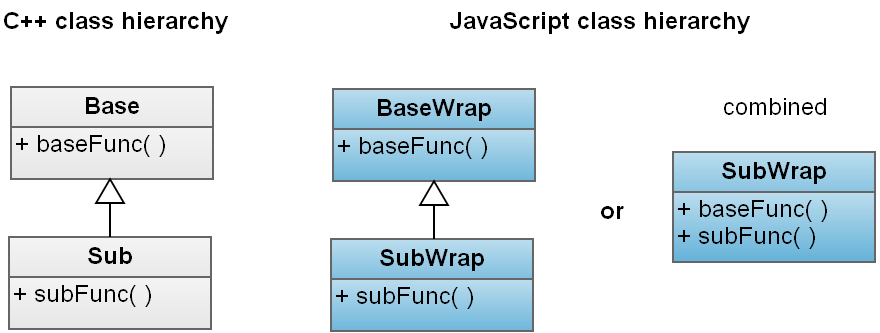
\includegraphics[scale=0.3]{Images/InheritanceWrapping.png}
	\caption{Wrapping inheritance chains}
	\label{fig:InheritanceWrapping}
\end{figure}

If base classes do not need to be exposed, multiple inheritance can be mimicked in the same way. Otherwise, if base classes are wrapped too, the subclass can inherit from one base class and borrow the properties from the others as explained in \myRefSection{sec:Mixins}.

problems with overwritten functions\todo{todo}

\subsection{Memory Management}

Memory management is probably the most problematic area in language binding and as such needed intensive research and thinking.\\
When bridging two programming languages, memory is often shared. This especially applies to instances of \myProperName{C++} classes that are wrapped for use in \myProperName{JavaScript}.

The \myProperName{JSAPI} user has to decide upon which side is responsible for freeing the memory - meaning which party holds the \textbf{ownership}. Depending on the application, this is not necessarily the party that allocated the memory.

There are basically three kinds of ownership.\\
For strict \textbf{script ownership}, the private data is always owned by the scripting language. The memory pointed to is freed, when the \mySCName{JSObject} is garbage collected (so, in the finalizer).\\
For strict \textbf{native ownership}, the memory is owned by the \myProperName{C++} library that is wrapped, which is thus responsible for freeing the private data. When a \mySCName{JSObject} with native ownership is garbage collected, the memory the private data points to is left unchanged.\\
\textbf{Mixed} ownership mixes both approaches. Ownership can be changed at run-time. Therefore, the \mySCName{JSObject} has to store state about who currently owns the private data. Functions for changing this state are exposed to script. When the \mySCName{JSObject} is garbage collected, the state is checked. If it is set to script ownership, the private data is freed. The ownership state can be saved along with the private data (for example in a struct that holds a \mySCName{void*} to the real private data and the state member) or in a reserved slot.

The glue code for wrapping a single class will generally make use one of these three abstract patterns, depending on how the user intends to use the class from script. As strict script and strict native ownership will apply to all wrapped objects (hence the term \textbf{strict}), the created \mySCName{JSObject}s do not need to store state of the ownership. The finalizer will be written according to the ownership.\\
Each kind of ownership comes with its own set of potential problems, which may occur depending on how the wrapped class and its instances are used.

\subsubsection{Potential Problems}

The two main problems are memory leaks and crashes/data-corruption because of dangling pointers (pointers that reference freed instances).

For this and the following section, the term \mySlang{C++ code} refers to the code of the library or application that is being wrapped - \textbf{excluding} the glue code, even though it is also written in \myProperName{C++}.

\textbf{Memory Leaks}

Memory leaks occur, when the ownership contract is not fulfilled. This happens mostly with classes that implement strict native ownership. Classes that implement a strict script ownership will delete the private data in the finalizer and thus will not lead to memory leak problems.

For mixed ownership, memory leaks generally occur when ownership was falsely handed over to \myProperName{C++}, indicating a bug in the script code.

A likely scenario for memory leaks to occur, are classes with native ownership that allow creating instances from script via \mySCName{new}. The constructor will allocate memory, but the finalizer will not free it. If such an instance is created from script, but the user forgets to pass it to the \myProperName{C++} code that is responsible for managing the memory, a leak will occur.\\
With native ownership, memory leaks also occur for functions returning stack-allocated copies. As explained in \myRefSection{sec:WrappingCopies}, new instances will be heap-allocated for wrapping. As ownership lies in the hands of \myProperName{C++}, these will never be freed.

\textbf{Dangling Pointers}

When using a dangling pointer, crashes (e.g. access violation) or data corruption are very likely - both of which cannot be caught or handled at run-time. Usage can happen in various ways: calling a member function of the (deleted) pointed object, accessing a field or trying to free the memory again.

It is not possible to detect a dangling pointer in \myProperName{C++}, as there is no way to check a non-\mySCName{NULL} pointer, whether it points to a valid instance in memory. Also, an instance has no knowledge about who references it, so it cannot inform the reference-holding entities about its deletion. If it could, these entities would simply set the reference to \mySCName{NULL}, which can be handled at run-time. But this is unfortunately not possible.\\
Smart pointers have been developed to overcome this lack and tackle dangling pointer problems, but they are only useful, when the whole application uses them, and not just the glue code.

Dangling pointers occur in several places. Deleted instances may be referenced by the \myProperName{C++} code of the wrapped library or by the private data of \mySCName{JSObject}s (thus, in the glue code). When using a dangling pointer, it makes no difference, which side falsely deleted or uses it.

For classes that have native ownership or objects that have their mixed ownership state set to \myProperName{C++}, a dangling pointer always indicates a problem in the application logic. The general rule should be known by any \myProperName{C++} programmer: if you delete an instance in your \myProperName{C++} code, do not use it afterwards - neither from \myProperName{C++} nor from script. If you do, crashes or data corruption are likely.\\
This rule applies equally to using a script owned instance in \mySCName{C++} code after the corresponding \mySCName{JSObject} has been garbage collected.

Another possible reason for a dangling pointer is the violation of the ownership contract. If a script owned object gets deleted by \myProperName{C++} code, the contract was ignored, indicating a bug in the program logic.

In terms of language binding, the consequences of using dangling pointers are \mySlang{acceptable}, when the dangling pointers result from bugs in the application logic (\myProperName{C++} or script). These dangling pointers are acceptable, because there is no way of preventing them in the glue code.

In certain situations, dangling pointers can occur, even though the user's code is correct on script and \myProperName{C++} side. Crashes and data-corruption in such cases is in no way acceptable (for the glue code writer), as it is not the user's fault. Systems have to be invented to prevent the existence or usage of such dangling pointers.\\
The problem occurs, when implementing strict script ownership for wrapped classes or when using objects that have their mixed ownership state set to script ownership. Given these prerequisites, dangling pointers can result from an existing \myProperName{C++} instance being wrapped by multiple \mySCName{JSObject}s (\mySlang{rewprapping}). When one of these \mySCName{JSObject}s is garbage collected, which in consequence frees the \myProperName{C++} instance, the private data of all the other \mySCName{JSObject}s will point to an deleted object. Using such a dangling pointer will lead to undefined behaviour like a crash or data-corruption. This will happen, when calling a function of one of the remaining \mySCName{JSObject}s or - at the latest - when the remaining objects are garbage collected and thus try to free the memory again. In any case, something will go wrong, when script owned objects are rewrapped.

\myRefListing{lst:DanglingCPP} and \myRefListing{lst:DanglingJS} illustrate the problem. The class \mySCName{SampleClass} has been exposed to \myProperName{JavaScript} as \mySCName{SampleClassWrap}, implementing script ownership and allowing construction. The functions from \myRefListing{lst:DanglingCPP} have also been wrapped.

\SingleSpacing
\begin{lstlisting}[language=C++, caption=Example for dangling pointers (\myProperName{C++}), label=lst:DanglingCPP]
SampleClass* cppSample = NULL;

void setSample(SampleClass* instPtr){ cppSample = instPtr; }
SampleClass* getSample()            { return  cppSample; }
SampleClass  getSampleCopy()        { return *cppSample; }
\end{lstlisting}
\OnehalfSpacing

\SingleSpacing
\begin{lstlisting}[language=JavaScript, caption=Example for dangling pointers (\myProperName{JavaScript}), label=lst:DanglingJS]
// creates new JSObject and C++ instance "cppInstance1"
var jsObj1 = new SampleClassWrap(); // points to "cppInstance1"

setSample(jsObj1); // cppSample points to "cppInstance1"

// creates new JSObject
var jsObj2 = getSample(); // points to "cppInstance1"

// wraps a copy (new C++ instance will be heap-allocated)
// creates JSObject and new C++ instance "cppInstance2"
var jsObj3 = getSampleCopy(); // points to "cppInstance2"
\end{lstlisting}
\OnehalfSpacing

In \myRefListing{lst:DanglingJS} \mySCName{jsObj1} and \mySCName{jsObj2} are two different \mySCName{JSObject}s pointing to the same \myProperName{C++} instance. One will hold a dangling pointer once the other has been garbage collected.\\
Functions that return copies (e.g. \mySCName{getSampleCopy}) will not lead to rewrapping as a new heap-allocated copy will be created for wrapping.

Looking at the given examples, it is clear that rewrapping can only happen when a \mySCName{JSObject} is retrieved from \myProperName{C++}, either through a property or  a non-copying function return. If a class is never used as an exposed field or as a pointer or reference function return, this kind of dangling pointers will not become a problem. Passing instances of such classes as parameters is generally unproblematic.

To prevent these dangling pointer problems, the glue code has to make sure that for every \myProperName{C++} instance that uses script ownership at most one \mySCName{JSObject} will be created. Rewrapping of script owned instances has to be prevented, for example by caching \mySCName{JSObject}s as explained in the next section.

\textbf{\myProperName{JavaScript} private data \mySCName{NULL} pointer}

A wrapped class may allow wrapping of \mySCName{NULL} pointers, resulting in the private data being set to \mySCName{NULL}. In such a case, the wrapper functions need to check the private data of the \mySCName{this} \mySCName{JSObject}. If it is \mySCName{NULL} a \myProperName{JavaScript} exception has to be thrown. Such a check is necessary, as calling a member function on a \mySCName{NULL} pointer produces undefined behaviour.

\subsection{Caching}

There are several ways of caching \mySCName{JSObject}s. Some are intrusive and require the original \myProperName{C++} code to be changed.

There are other good reasons for performing caching, besides prevention of dangling pointers.\\
Depending on the implementation, a caching system may perform better than recreating \mySCName{JSObject}s for the same \myProperName{C++} instance all over again.\\
Associating a single \mySCName{JSObject} with one \myProperName{C++} instance  also makes it possible to add information to the \mySCName{JSObject} that persists, when crossing the language border  multiple times in both directions. That way, the script user is able to add additional properties to the particular instance and retrieve those at any time.

\subsubsection{Value Properties}

As explained in \myRefSection{sec:ValueProperties}, fields can be wrapped and defined on the \mySCName{JSObject} directly. If the same field is not exposed in any other way and the instance the field belongs to is never rewrapped, then the field's wrapper \mySCName{JSObject} is effectively cached.

\subsubsection{Cache Maps}

One way of caching \mySCName{JSObject}s is to store the first created \mySCName{JSObject} in a map along with the memory address of the instance that is wrapped. Whenever the same instance needs to be wrapped, the map is checked for the memory address and if an entry exists, the corresponding \mySCName{JSObject} will be used instead of rewrapping the \myProperName{C++} instance. However, there are several drawbacks with this approach.

\mySCName{JSObject}s with script ownership can simply remove their corresponding entry from the cache map, when they are garbage collected. But for objects that are wrapped with native ownership, the glue code has no notion of knowing, when the \myProperName{C++} instance has been deleted. Thus, all \mySCName{JSObject}s in the cache map need to be kept alive until the end of the application, wasting valuable memory. As native ownership does not result in the \mySlang{unacceptable} dangling pointer problem that occurs when rewrapping, the cache maps could safely be cleaned from time to time. With this approach, rewrapping can occur, but is less likely.\\
Either way, problems with \mySlang{cuckoo pointers} are possible for wrapped classes that use native ownership. A cuckoo pointer was originally an ordinary pointer to an existing object. The object was deleted, turning the pointer into a dangled pointer. Coincidentally a new object of an arbitrary type was allocated at the same memory position. If a cache map contains an entry for the original pointer and a cuckoo pointer with the same memory position is looked up after the original instance has been destroyed, the cache map will return the old \mySCName{JSObject}, which still has a dangling pointer to the deleted instance. Using this \mySCName{JSObject} will result in undefined behaviour. To prevent this, type information can be saved along with the memory address and compared upon lookup. This will ensure that at least the \mySCName{JSObject} is of the same class and using the cuckoo pointer is thus safe.

When it comes to multiple inheritance, memory address and object do not have a 1 to 1 correlation. Because of pointer fixup, casting a subclass pointer to one of its base classes will result in different memory positions depending on which base class it was casted to. Though this is a very unlikely scenario, it is possible that due to different memory positions, multiple \mySCName{JSObject}s may be created for the same instance.

\subsubsection{KnowledgeJS}

\mySlang{KnowledgeJS}, what I call it, is another kind of caching that also stores a mixed ownership state.

This caching system is intrusive, meaning that the \myProperName{C++} classes, that are wrapped, need to be modified by inheriting from the \mySCName{KnowledgeJS} class, which implements most features.

In this system, the \myProperName{C++} instance stores a pointer to the \mySCName{JSObject} that it is being wrapped by. At the same time, the \mySCName{JSObject} stores the \myProperName{C++} instance in its private data as usual. Thus, both have knowledge about each other, as they are in a 1 to 1 relationship.

When the \myProperName{C++} instance needs to be wrapped, it is checked if it already has a \mySCName{JSObject} associated. If so, this \mySCName{JSObject} is used and can be handed to script. If not, a new \mySCName{JSObject} is created and both are connected.

If the object has script ownership, it will delete the \myProperName{C++} instance upon garbage collection.\\
For native ownership, the \mySCName{JSObject} has to be kept alive as long as the \myProperName{C++} instance is. \myProperName{SpiderMonkey} provides functionality for rooting \mySCName{JSObject}s so that they are not garbage collected. Upon destruction of the \mySCName{C++} instance, the corresponding \mySCName{JSObject} will be unrooted and its private data set to \mySCName{NULL}. As wrapped member functions check for private data being \mySCName{NULL}, \myProperName{JavaScript} exceptions will be thrown, when the \mySCName{JSObject} is used from script after the destruction of the C++ \mySCName{instance}. This is better than having a dangling pointer, which would lead to undefined behaviour.

\mySlang{KnowledgeJS} is the most elegant way of wrapping and caching, as there are no restrictions of how a type can be used and no undefined behaviour to be expected. But because of its intrusiveness it can not be used to wrap already existing libraries without modification.

\subsection{Const}

Being a weakly typed language, \myProperName{JavaScript} has no notion of \mySCName{const} values. As such, \mySCName{const} class instances are wrapped as non-\mySCName{const}. This removes security, when trespassing the language border and may lead to wrapped instances being used in an unexpected or unintended fashion.

It is free to the \myProperName{JSAPI} user to only expose constant functions of a class.

It is also possible to save a \mySCName{const} state in the \mySCName{JSObject} itself. Wrapper functions could check this state. If it is \mySCName{true} and a non-\mySCName{const} member function is used, a \myProperName{JavaScript} exception could be thrown.\\
This concept is not feasible, when caching \mySCName{JSObject}s. If a \myProperName{C++} function returns an instance for which a cached \mySCName{JSObject} exists and sets its \mySCName{const} state to \mySCName{true}, then all other users that were previously using the \mySCName{JSObject} in a non-\mySCName{const} manner will suddenly receive exceptions. This has to do with the \mySCName{const} state being stored in the value (the object) instead of the variable.

\section{Global Variables}

Global variables are wrapped similarly to class fields as described in \myRefSection{sec:Fields}. Instead of defining the property on class prototype or instances, it is defined on the global \myProperName{JavaScript} object or the \mySCName{JSObject} that represents the corresponding namespace.

\section{Typedefs}

As one of the main purposes of typedefs is to assign a simple name for a \myProperName{C++} type to ease code writing, a typedef feature is less needed in weakly typed languages.

To achieve a typedef-like effect in \myProperName{JavaScript}, constructor functions can be defined as properties on multiple objects, even with different property names.\\
It has to be pointed out, that there is no equivalent of typedefs for primitive types (except for \mySCName{null} and \mySCName{undefined}, as these are a value and type at the same time).

\section{Function Pointers and Callbacks}

\SingleSpacing
\begin{lstlisting}[language=C++, caption=\myProperName{C++} function that takes a function pointer]
void someFunc(float (*funcPointer)(int));
\end{lstlisting}
\OnehalfSpacing

\myProperName{C++} functions that take function pointers, often referred to as callbacks, are a problematic topic.\\
Two cases need to be distinguished:
\begin{enumerate}
\item Passing \myProperName{C++} functions as callbacks
\item Passing script functions as callbacks
\end{enumerate}

\subsection{Passing \myProperName{C++} Functions as Callbacks}

The first case is unproblematic. A pointer to a \myProperName{C++} function can be wrapped inside a simple \mySCName{JSObject}, by casting the function pointer (function address) to a \mySCName{void} pointer and saving it as the private data of the \mySCName{JSObject}. The glue code for the function that takes the function pointer will retrieve the function pointer from the private data of the appropriate argument by casting it back to the appropriate function type.

\subsection{Passing Script Functions as Callbacks}

\myProperName{JavaScript} functions can not simply be passed as a function pointer. When passing a \myProperName{JavaScript} function as a callback, a wrapper function that has the same function type as the pointer has to be created. This is the \myProperName{C++} function that will then be passed to the function that takes the function pointer. Inside, the \myProperName{C++} arguments must be converted to types that \myProperName{JavaScript} understands. The \myProperName{JavaScript} callback-function has to be called and its return value converted to the \myProperName{C++} type that the function type expects. Thus, such a wrapper function works the exact other way around than wrapper functions presented earlier in this chapter:

\SingleSpacing
\begin{lstlisting}[language=C++, caption=Wrapper code for handling methods that take function pointers \#1]
float wrapper_callback(int param)
{
	// 1. convert param to JavaScript Number
	// 2. call the JavaScript function
	// 3. convert the return value from a JS Number to float
}

JSBool wrapper_someFunc(JSContext *cx, uintN argc, jsval *vp)
{
	// call someFunc
	someFunc(&wrapper_callback);
}
\end{lstlisting}
\OnehalfSpacing

This approach comes with one big problem, when calling \mySCName{someFunc} multiple times with different \myProperName{JavaScript} callbacks: As \mySCName{wrapper\_callback} is a simple \myProperName{C++} function created at compile-time, it has no notion of state and as such no information about which \myProperName{JavaScript} function to use as the callback.

One way around this, is to save the \myProperName{JavaScript} callback function passed to \linebreak\mySCName{wrapper\_someFunc} in a global variable, so it can be retrieved within \mySCName{wrapper\_callback}. This approach only works, when the callback is called during the execution of \mySCName{someFunc}. If it is called at a random point in program execution, \mySCName{wrapper\_callback} would use the last \myProperName{JavaScript} function that was saved in the global variable, which may not be the one the user intended to be called. Even if the global variable was a collection like a queue to which every \myProperName{JavaScript} function was pushed when calling \mySCName{wrapper\_someFunc} and dequeued upon \mySCName{wrapper\_callback}, the result would be dependent on the order of execution. Thus this work-around is highly suboptimal.\\
An example to illustrate the wrong behaviour: The script user declares two \myProperName{JavaScript} functions, one printing the string \mySCString{Hello}, the other \mySCString{World} and passes them to \linebreak\mySCName{callLater}, which takes a time delay:

\newpage
\SingleSpacing
\begin{lstlisting}[language=JavaScript, caption=Passing a callback function]
callLater(10, function(){ print("Hello"); }); // call in 10 seconds
callLater(5,  function(){ print("World"); }); // call in 5  seconds

// time passes
// 5 seconds later : "Hello"
// 10 seconds later: "World"
\end{lstlisting}
\OnehalfSpacing

The result should be the other way around, because the time delay for \mySCString{Hello} is 10 and thus after \mySCString{World}.

\textbf{Passing state information}

Without run-time function creation (more about that later), a function callback of the given form can not be resolved in any other way then the previously presented. To support calling \mySCName{someFunc} multiple times with different callbacks, state information needs to be provided. This is possible in two ways, both of which need modification of the original function and/or parameter declaration.

State information can be provided by extending \mySCName{someFunc} and the function type to take an additional \mySCName{void} pointer for user data. The script function is then passed as user data to \mySCName{someFunc}, which will use/save it along with the function pointer. The user data will be passed as the \mySCName{void} pointer to the \myProperName{C} callback function and as such can be used in \mySCName{wrapper\_callback} to retrieve the script function to call.

\SingleSpacing
\begin{lstlisting}[language=C++, caption=Wrapper code for handling methods that take function pointers \#2]
void someFunc(float (*funcPointer)(int, void*), void* data);

float wrapper_callback(int param, void* data)
{
	// 1. convert param to JavaScript Number
	// 2. retrieve JSFunction to call from data
	// 3. call the JavaScript function
	// 4. convert the return value from a JS Number to float
}

JSBool wrapper_someFunc(JSContext *cx, uintN argc, jsval *vp)
{
	// retrieve JSFunction* from vp
	jsval* args = JS_ARGV(cx, vp);
	void* funcPtr =  jsval_to_jsfunction(cx, args[0]);
	
	// call someFunc
	someFunc(&wrapper_callback, funcPtr);
}
\end{lstlisting}
\OnehalfSpacing

Another way to modify the original \mySCName{someFunc} is to let it take functors that contain state information instead of a function pointer. Instead of passing the \mySCName{JSFunction} as an additional \mySCName{void} pointer, it would be saved in the functor object.

Either way, passing state information demands modification of the original source code. This may prove to be impossible in cases where 3rd party libraries are used.

\textbf{Run-time function creation and closures}

\myProperName{C++11} allows the creation of functions at run-time with the help of lambda functions\footnote{Lamdba functions: \url{http://www.cprogramming.com/c++11/c++11-lambda-closures.html}}. Lamdba functions can capture state and thus seem to be capable of solving the given problem. This concept is also known as a closure and, as a side note, is very common in \myProperName{JavaScript}.
\\Unfortunately only state-less lamdba functions can be passed as function pointers. Lambda functions that capture state are only syntactic sugar for functors and as such can not be used to solve the given problem.

The only other way of creating functions at run-time is to create the machine-code itself at run-time. This, of course, requires assembly and is thus outside of portable \myProperName{C++}. With this method, the memory address of the \myProperName{JavaScript} function to call could simply be stored in the machine-code itself.

\myProperName{libffi}\footnote{\myProperName{libffi}: \url{http://sourceware.org/libffi/}} contains functionality for creating these types of closures at run-time. It is used by \myProperName{Mozilla}'s \myProperName{js-ctypes} for allowing \myProperName{JavaScript} functions to be passed as \myProperName{C} function pointers. \myProperName{Python}'s \myProperName{ctypes} uses it for the same reason. As the creation of closures is a highly machine-dependent operation, it is indispensable to use a 3rd party like \myProperName{libffi}.

The creation of machine-code at run-time is the only way for completely supporting script functions as callbacks. It has the drawback of an additional library dependency and is also not supported on all platforms.

\section{Arrays and Collections}

Arrays and collections like \mySCName{std::vector} can be converted to \myProperName{JavaScript} arrays. Maps, that use strings for the keys, can be converted to ordinary \myProperName{JavaScript} objects, which are basically hashmaps.

When doing these conversions, the single members need to be wrapped and added to the \myProperName{JavaScript} array. As a new \myProperName{JavaScript} container is created, changing this container (e.g. adding or removing elements) from script will not effect the original \myProperName{C++} container. If such a behaviour is necessary, the collection class (e.g. \mySCName{std::vector}) needs to be wrapped itself. To make it look more natural in \myProperName{JavaScript}, the interface can be created in a way that resembles \myProperName{JavaScript} arrays.

\section{Templates}

Templates are an advanced feature of \myProperName{C++} for writing classes that can use arbitrary types. As such, templates are not really needed in weakly typed dynamic languages like \myProperName{JavaScript}.

Templates are merely blueprints for classes (and functions) that are instantiated at compile-time with the given types. This happens either implicitly or or explicitly.\\
Being a compile-time feature, generic templated classes like \mySCName{std::vector<T>} cannot be wrapped and thus made usable from script with arbitrary types set for the template parameters (e.g. \mySCName{T}).\\
As template instantiations (e.g. \mySCName{std::vector<int>}) are ordinary classes, they can be wrapped like any other. This means that for any type that the \myProperName{SpiderMonkey} user might want to use as a template parameter, the corresponding template needs to be instantiated and wrapped in the glue code. Being individual classes, instantiated templates have no relationship to each other and thus such each instantiation needs to be wrapped on its own.\\
Glue code can be shared, by using templated wrapper functions though: 

\SingleSpacing
\begin{lstlisting}[language=C++, caption=A templated JSNative]
template<T>
float getFloat(T param1);

template<T>
JSBool getFloat_wrapper(JSContext *cx, uintN argc, jsval *vp)
{
	// code that uses T
}

JSFunction* func = JS_DefineFunction(context, someJSObject,
        "getFloat",             // name of the function
        getFloat_Wrapper<int>,  // wrapper function instantiation
        1, JSPROP_ENUMERATE);
\end{lstlisting}
\OnehalfSpacing

\section{Generic Wrapper}
\label{sec:GenericWrapper}
Sometimes the user does not need class members to be exposed to script, but only wants to pass instances across the language border. The user might for example receive a wrapped instance from an exposed \myProperName{C++} function and pass it on to another \myProperName{C++} function, without using the \myProperName{JavaScript} object in between.

As no members are exposed, it is possible to use the same \mySCName{JSClass} for all kinds of instances. This generic wrapper will leave ownership to \myProperName{C++}.\\
In contrast to the previously explained wrapping of classes, the \mySCName{JSClass} \mySCName{GenericWrapper} will not be bound to a specific type of private data and as such can not be used for type checking. Thus, type information needs to be stored along with the private data \mySCName{void*}.

There are several ways to do this, for example the \myProperName{C++} \mySCName{typeid}\footnote{\mySCName{typeid}: \url{http://www.cplusplus.com/reference/std/typeinfo/type_info/}} operator, which returns the type information of a given value. Though \mySCName{type\_info}s can be compared, they have no knowledge about inheritance chains.\\
There is a proposal to support rich pointers\footnote{Rich pointer proposal: \url{http://www.open-std.org/jtc1/sc22/wg21/docs/papers/2012/n3340.pdf}} (pointers that also contain type information) in \mySCName{C++}, but it is uncertain if the idea of rich pointers will ever become part of a new \myProperName{C++} standard.

During research I came across \myAuthorName{Cassio Neri}'s concept of an \mySCName{any\_ptr} - a class that holds a pointer and its type information. \mySCName{any\_ptr} allows casting up and down in inheritance chains at run-time without the possibility of crashes. If an \mySCName{any\_ptr} cannot be casted to a given type, its \mySCName{cast} function simply returns \mySCName{NULL}. An important feature is its support for classes without RTTI.

\begin{lstlisting}[language=C++, caption=Implementation of \mySCName{any\_ptr}]
class any_ptr {
    void* ptr_;
    void (*thr_)(void*);
 
    template <typename T>
    static void thrower(void* ptr) { throw static_cast<T*>(ptr); }
 
public:
    template <typename T>
    any_ptr(T* ptr) : ptr_(ptr), thr_(&thrower<T>) {}
 
    template <typename U>
    U* cast() const {
        try { thr_(ptr_); }
        catch (U* ptr) { return static_cast<U*>(ptr); }
        catch (...) {}
        return 0;
    }
};

std::string str;
any_ptr anyPtr(&str); // T is deduced from &str

std::string* strPtr = anyPtr.cast<std::string>(); // --> points to str
std::exception* ePtr = anyPtr.cast<std::exception>(); // --> NULL
\end{lstlisting}
\OnehalfSpacing

The concept is simple, but clever. Along with the pointer as \mySCName{void*}, the \mySCName{any\_ptr} stores the address of a template function instantiation (\mySCName{thrower}) that was instantiated with the known type of the pointer (e.g. \mySCName{std::string}). This function does nothing but throw the casted pointer as an exception. The \mySCName{cast} function is another template function that takes the type that the pointer should be casted to as the template parameter \mySCName{U} (for example \mySCName{std::string}, \mySCName{std::exception}, \mySCName{int}, etc.). This type will be used in a \mySCName{catch} clause to catch the pointer that was thrown in \mySCName{thrower}. If the \mySCName{catch} clause can catch the exception the cast is successful and the casted pointer returned. Otherwise \mySCName{NULL} is returned. Catching a \mySCName{U*} will also catch any subclass of the type used for \mySCName{U}.

Instead of storing the instance pointer directly, \mySCName{GenericWrapper} will store an instance of \mySCName{any\_ptr}, which was created with \mySCName{new any\_ptr(instancePtr)}. 

Using the run-time exception system has surely worse performance and storing an \mySCName{any\_ptr} as the private data adds one level of indirection compared to storing the instance pointer itself. Nevertheless, \mySCName{any\_ptr} seems to be the only type-safe way of casting unknown private data.

As \myProperName{C++} holds ownership, the generic wrapper should not be used for wrapping function return values that are copies, as the memory will be leaked.

\section{Error Handling}
\label{sec:ErrorHandling}

Errors can occur in a lot of places. Converting a parameter to the expected type might fail. The \myProperName{C++} code that is called may throw an exception.

The \myProperName{JavaScript} engine does not automatically handle exceptions. The \myProperName{JSAPI} user has to do this himself at the language border - meaning the glue code and the wrapper functions. When a wrapper function returns \mySCName{false}, it tells the virtual machine that an error occurred and an exception has been set. Setting exceptions can be done using \mySCName{JS\_ReportError}:

\SingleSpacing
\begin{lstlisting}[language=C++, caption=Error handling at the language border]
JSBool some_wrapper(JSContext *cx, uintN argc, jsval *vp)
{
	try {
		// code that throws exception
		
	} catch(std::exception& e) {
		JS_ReportError(cx, e.what());
		return false;
	} catch(...) {
		JS_ReportError(cx, "some_wrapper: An unknown exception occurred");
		return false;
	}
	
	// no errors detected
	return true;
}
\end{lstlisting}
\OnehalfSpacing

\section{Accessing \myProperName{JavaScript} Objects from \myProperName{C++}}

This chapter mostly focused on exposing \myProperName{C++} functionality to \myProperName{JavaScript}.

\myProperName{SpiderMonkey} also provides functions for getting and accessing \myProperName{JavaScript} objects and values. Object properties can be inspected and functions called.

\mySCName{JS\_GetProperty} can be used to access the property of a \mySCName{JSObject}. The values stored in properties can be unwrapped in the presented way to access the wrapped \myProperName{C++} instances. Type checking has to be performed to verify the data coming from \myProperName{JavaScript}.

The functionality to access arbitrary \myProperName{JavaScript} objects and calling \myProperName{JavaScript} functions from \myProperName{C++} makes it possible to use \myProperName{JavaScript} libraries from native code.